\section{Iteración 2}
\label{sec:iteracion_2}

Después de que finalizó la primera iteración y ya que todas las pruebas pasaron exitosamente, se continúa con la segunda iteración.


\subsection{Iteration Planning Meeting}
\label{sub:iteration2_planning_meeting}


Al igual que la primera iteración, las fases de exploración y planeación se realizan al mismo tiempo, en el sentido que no es necesario repartir las tareas resultantes de la exploración, por lo tanto al mismo tiempo en que se determinan las tareas se puede realizar la estimación de las mismas.

  \subsubsection{Exploración y Planeación}
  \label{subs:iteration2_exploracion_planeacion}

  Para la segunda iteración se toman en cuenta todas las historias de usuario restantes, y de acuerdo al criterio de escoger las siguientes historias más relevantes y de mayor valor para el producto, se escogió la historia de usuario US03 y US04.\\

  Al igual que en la primera iteracion se toman las historias de usuario y las dividimos en las Tareas de Ingeniería, las cuales serán trabajadas en la fase de la Implementación.

  \subsection{Tareas del US03}
  \label{sub:us03_tasks}

    \begin{table}[H]
  \begin{center}
    \begin{tabularx}{\textwidth}{ c  X  C{2.3cm} }
      \toprule
        \textbf{Código} &
        \multicolumn{1}{c}{\textbf{Tarea}} &
        \textbf{Estimación [dias]}\\

      \midrule
      %   RF011
      %   &
      %   % Crear un archivo shapefile con información inicial de lugares principales dentro el campus de la UMSS.
      %   &
      %   2 \\
      %
      % \addlinespace
      %   RF012
      %   &
      %   % Preparar la base de datos para manejar información geográfica de rutas.
      %   &
      %   1 \\

      % \addlinespace
        T013
        &
        Investigar e instalar una herramienta que permita usar un servicio de mapas.
        &
        1 \\

      \addlinespace
        T014
        &
        El usuario puede ver un mapa del campus de la UMSS.
        &
        0.5 \\

      \addlinespace
        T015
        &
        El usuario puede ver un marcador sobre el lugar.
        &
        0.5 \\

      \addlinespace
        T016
        &
        El marcador tiene información básica del lugar, por ejemplo el nombre y el piso.
        &
        0.5 \\

      % \addlinespace
      %   T017
      %   &
      %   % El usuario puede ver un marcador mostrando el lugar actual donde se encuentra (el usuario).
      %   &
      %   0.5 \\
      %
      % \addlinespace
      %   T018
      %   &
      %   % Desarrollar un módulo que encuentra la ruta más corta usando la base de datos con información geográfica ruteable de RF012.
      %   &
      %   2 \\
      %
      % \addlinespace
      %   RF019
      %   &
      %   % El usuario puede ver una línea roja que une el marcador de la posición del usuario con el marcador del lugar.
      %   &
      %   1 \\

      \addlinespace
        TS003
        &
        Crear pruebas de funcionalidad del US04.
        &
        1 \\

      \addlinespace
      \midrule
        & \multicolumn{1}{R{7cm}}{\textbf{Total: }}
        & 10 \\

      \bottomrule
    \end{tabularx}
    \caption{Tareas del US04}
    \label{tab:us04_tasks}
  \end{center}
\end{table}



  \subsection{Tareas del US04}
  \label{sub:us04_tasks}

    \begin{table}[H]
  \begin{center}
    \begin{tabularx}{\textwidth}{ c  X  C{2.3cm} }
      \toprule
        \textbf{Código} &
        \multicolumn{1}{c}{\textbf{Tarea}} &
        \textbf{Estimación [dias]}\\

      \midrule
        T011
        &
        Crear un archivo shapefile con información inicial de lugares principales dentro el campus de la UMSS.
        &
        2 \\

      \addlinespace
        T012
        &
        Preparar la base de datos para manejar información geográfica de rutas.
        &
        1 \\
      %
      % \addlinespace
      %   T013
      %   &
      %   Investigar e instalar una herramienta que permita usar un servicio de mapas.
      %   &
      %   1 \\

      % \addlinespace
      %   T014
      %   &
      %   El usuario puede ver un mapa usando un servicio del campus de la UMSS.
      %   &
      %   0.5 \\

      % \addlinespace
      %   T015
      %   &
      %   El usuario puede ver un marcador sobre el lugar.
      %   &
      %   0.5 \\
      %
      % \addlinespace
      %   T016
      %   &
      %   El marcador tiene información básica del lugar, nombre, piso.
      %   &
      %   0.5 \\

      \addlinespace
        T017
        &
        El usuario puede ver un marcador mostrando el lugar actual donde se encuentra (el usuario).
        &
        0.5 \\

      \addlinespace
        T018
        &
        Desarrollar un módulo que encuentra la ruta más corta usando la base de datos con información geográfica ruteable de T012.
        &
        2 \\

      \addlinespace
        T019
        &
        El usuario puede ver una línea roja que une el marcador de la posición del usuario con el marcador del lugar.
        &
        1 \\

      % \addlinespace
      %   TS003
      %   &
      %   Crear pruebas de funcionalidad del US04.
      %   &
      %   1 \\

      \addlinespace
      \midrule
        & \multicolumn{1}{R{7cm}}{\textbf{Total: }}
        & 10 \\

      \bottomrule
    \end{tabularx}
    \caption{Tareas del US04}
    \label{tab:us04_tasks}
  \end{center}
\end{table}



  \subsection{Calendario de Entregas}
  \label{subs:schedule_2}

    % \begin{table}[!ht]
%
% \end{table}
\begin{table}[H]

  \begin{center}

\begin{ganttchart}[
  canvas/.append style={fill=none, draw=black!5, line width=.75pt},
  hgrid style/.style={draw=black!5, line width=.75pt},
  vgrid={*1{draw=black!5, line width=.75pt}},
  %today=0,
  % today label=Semana 3,
  today rule/.style={
    draw=black!64,
    dash pattern=on 3.5pt off 4.5pt,
    line width=1.5pt
  },
  today label font=\small\bfseries,
  title/.style={draw=none, fill=none},
  title label font=\bfseries\footnotesize,
  title label node/.append style={below=7pt},
  include title in canvas=false,
  bar label font=\mdseries\small\color{black!70},
  bar label node/.append style={left=2cm},
  bar/.append style={draw=none, fill=black!63},
  bar incomplete/.append style={fill=barblue},
  bar progress label font=\mdseries\footnotesize\color{black!70},
  group incomplete/.append style={fill=groupblue},
    group left shift=0,
    group right shift=0,
    group height=.5,
    group peaks tip position=0,
    group label node/.append style={left=.6cm},
    group progress label font=\bfseries\small,
    link/.style={-latex, line width=1.5pt, linkred},
    link label font=\scriptsize\bfseries,
    link label node/.append style={below left=-2pt and 0pt},
  ]{1}{12}
  \gantttitle{Calendario de Entregasde de la Iteración 2}{7} \\[grid]
  \gantttitle{Semana 1}{7}
  \gantttitle{Semana 2}{7} \\
  % \gantttitle{Noviembre}{4} \\
  \gantttitle[title label node/.append style={below left=7pt and -3pt}]{D\'ia:\quad15}{0}
  \gantttitlelist{16,...,30}{1} \\
  % \ganttgroup[progress=0]{Historias de Usuario}{1}{8} \\
  \ganttbar[
    progress=0,
    name=bar1
  ]{\textbf{User Story 04}}{1}{12} \\
  % \ganttbar[
  %   progress=0,
  %   name=bar2
  % ]{\textbf{User Story 03}}{10}{12} \\
  % \ganttbar[
  %   progress=0,
  %   name=bar3
  % ]{\textbf{Iteración 3}}{5}{6} \\
  % \ganttbar[
  %   progress=0,
  %   name=bar4
  % ]{\textbf{Iteración 4}}{7}{8} \\
  % \ganttbar[
  %   progress=100,
  %   name=bar5
  % ]{\textbf{Actividad 5}}{5}{7} \\
  % \ganttbar[
  %   progress=80,
  % ]{\textbf{Actividad 6}}{8}{8} \\
  % \ganttbar[
  %   progress=49,
  % ]{\textbf{Actividad 7}}{9}{11} \\
  % \ganttmilestone{Hito 1}{11}{11}  \\
  % \ganttmilestone{Hito 2}{12}{12} \\
  %

  % \ganttmilestone{Q6 report}{24}{24} \\
  % \ganttmilestone{M1: Project finished}{8}{8}

  % \ganttlink[link type=f-s]{bar1}{bar2}
  % \ganttlink[link type=f-s]{bar2}{bar3}
  % \ganttlink[link type=f-s]{bar3}{bar4}

\end{ganttchart}

\caption{Calendario de Entregas de la Iteración 2}
\label{tab:calendario_entregas_iteracion_2}

\end{center}
\end{table}



\subsection{Implementación}
\label{sub:implementacion_iteracion_2}

% Durante esta fase es donde se implementaran las tareas especificadas en la tabla \ref{tab:us04_tasks}.

    


% movido a implementacion - iteracion 2
\subsubsection{Geolocalizar los Lugares}
\label{sub:fronted_lugares}



Un ``lugar'' tienen almacenada en la base de datos su posición georreferenciada, por lo tanto la aplicación necesita mostrar un lugar o geolocalizarlo sobre un mapa. Para resolver esta tarea se utilizó \emph{ember-leaflet}, una librería creada para manipular mapas y diseñada especialmente  para su implementación en dispositivos móviles.\\

Para instalar esta librería solo se necesita ejecutar el siguiente comando y posteriormente ya se puede empezar a utilizarla.\\

\begin{verbatim}
 $ ember install ember-leaflet
\end{verbatim}


Primeramente es necesario conocer las coordenadas del ``lugar'', para lo cual se hara un \emph{request} al API de la aplicación para obtener la información del ``lugar'', el URI designado para esta tarea es \verb|places/:id| usando el verbo HTTP \emph{GET}, para mejorar el manejo de la coordenadas se utilizo el formato \emph{GeoJSON}, las coordenadas son procesadas dentro del \emph{controlador} de ember que pasa los valores necesarios al \emph{template}, tal como se puede observar en el siguiente codigo, los atributos de \emph{lat} y \emph{lng} son la latitud y longitud respectivamente, es la combinación de ambos da el punto georerenciado donde se encuentra ubicado el lugar, para un mejor visualizacion se esta usando esta locación para centrar la ubicación del  mapa. Se puede notar que el \emph{tag} \verb|leaflet-map| es un componente personalizado, perteneciente a \emph{ember-leaflet}, es donde se inicializa el mapa en este caso \emph{Open Street Maps}, como se puede apreciar en la figura \ref{fig:ember_leaflet}.


% \begin{center}
%   \begin{verbatim}
%     var maker = new google.maps.Marker({
%       position: new google.maps.LatLng( lat, lng  )
%       map: UMSS.map
%     });
%   \end{verbatim}
% \end{center}

\begin{verbatim}
  {{#leaflet-map lat=lat lng=lng zoom=zoom}}
    {{tile-layer url="http://{s}.tile.openstreetmap.fr/hot/{z}/{x}/{y}.png" }}
      {{#marker-layer location=location}}
        <h3>{{model.name}}</h3>
        {{model.description}} <br>
        <strong>telf:</strong> {{model.phone}} <br>
        <strong>piso </strong>#{{model.level}}
    {{/marker-layer}}
  {{/leaflet-map}}
\end{verbatim}


\begin{figure}[H]
      \begin{center}
        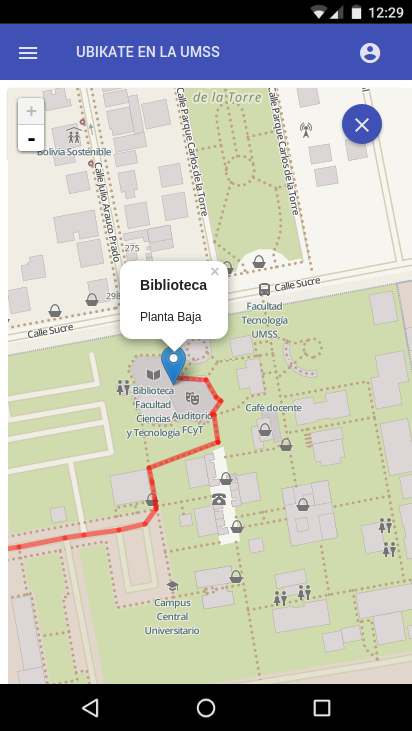
\includegraphics[width=0.3\textwidth]{ember_leaflet}

        % \caption{\emph{ember-leaflet} nos ayuda a desplegar un mapa y mostrar un \emph{punto} o \emph{lugar} con un \emph{marcador} y dibuja una línea de color rojo sobre el mapa.}
        \caption{ Mapa mostrado con la ayuda de \emph{ember-leaflet}}
        \label{fig:ember_leaflet}
        \caption*{Fuente: Elaboración propia.}
      \end{center}
\end{figure}

\emph{Ember-leaflet} se encarga de geolocalizar un punto georreferenciado sobre un mapa y también permite personalizarlo, por ejemplo se puede añadir un \emph{marcador}  y personalizarlo con el \emph{tag} \verb|#marker-layer| e incluir los demás datos obtenidos del backend, como se puede apreciar en la figura \ref{fig:baquita_place}.


\begin{figure}[H]
  \begin{center}
    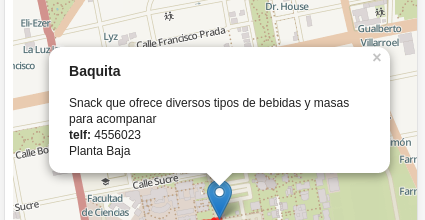
\includegraphics[width=0.8\textwidth]{iteration2/baquita_place}
    \caption{Tooltip con la información de un lugar.}
    \label{fig:baquita_place}
    \caption*{Fuente: Elaboración propia.}
  \end{center}
\end{figure}


% Para poder acceder a la anterior vista, es necesario en primer lugar seleccionarlo de una lista





% \begin{figure}[H]
%  \begin{center}
%    \caption{Vista de la lista de Lugares registrados en el sistema.}
%    \label{fig:places_index}
%    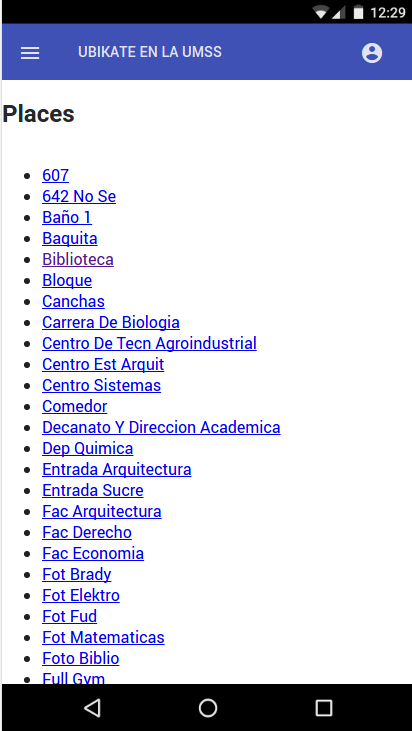
\includegraphics[width=0.5\textwidth]{iteration1/places_index}
%    \caption*{Fuente: Elaboración propia}
%  \end{center}
% \end{figure}


% \begin{figure}[H]
%  \begin{center}
%    \caption{Vista de la búsqueda de lugares a través de un cajón de búsqueda.}
%    \label{fig:places_search}
%    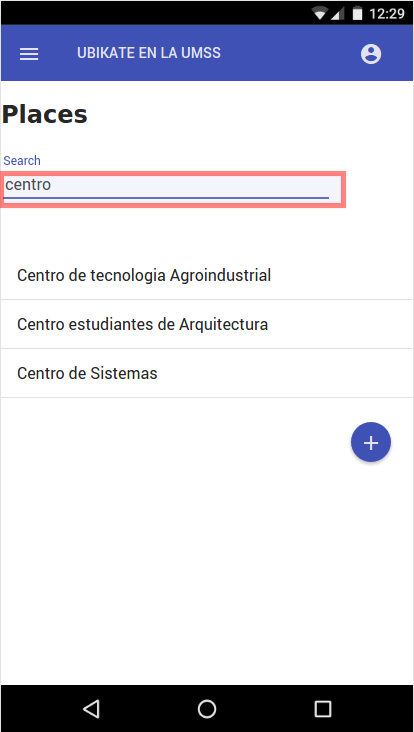
\includegraphics[width=0.5\textwidth]{iteration1/places_search}
%    \caption*{Fuente: Elaboración propia}
%  \end{center}
% \end{figure}


% Para implementar esta funcionalidad del sistema fue necesario utilizar las funcionalidad de Ember JS.
%
% \begin{verbatim}
%  {{#paper-item class="md-1-line" onClick=(transition-to 'places.show' place)}}
%      <div class="md-list-item-text">
%          <span>{{place.name}}</span>
%      </div>
%  {{/paper-item}}
% \end{verbatim}
%
%
% \begin{figure}[H]
%    \label{fig:place_show}
%    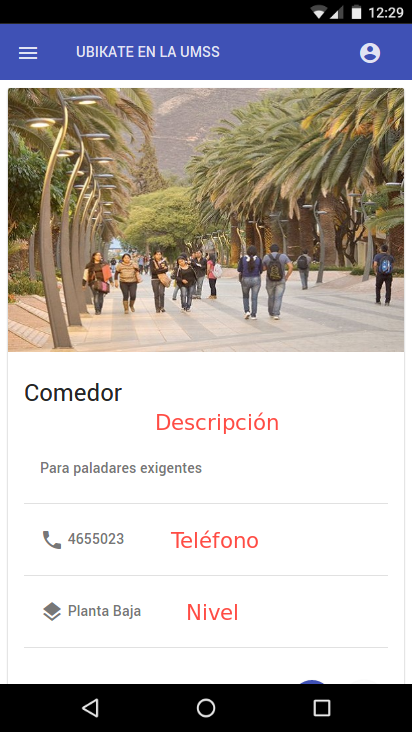
\includegraphics[width=0.5\textwidth]{iteration1/place_show}
%    \caption*{Fuente: Elaboración propia}
%  \end{center}
% \end{figure}

% movido a implementacion - iteracion 2


\subsubsection{Geolocalizar los Usuarios}
\label{sub:Manejo de Usuarios}

Si se quiere saber la ruta más corta entre el usuario y un lugar, es necesario conocer la locación del usuario y hay que tomar en cuenta que esta información no se encuentra en la base de datos. Por lo tanto es necesario obtener el punto georreferenciado del usuario como punto de inicio de la ruta mas corta, para lo cual se utilizó el API de geolocalización propio de HTML5, la especificación de HTML5 indica que el navegador puede acceder y usar los recursos nativos de un smartphone pero es necesaria la aceptación del usuario mediante un mensaje que el navegador despliega, la locación es encontrada mediante la triangulación de Coordenadas por GPS (el mas exacto a la hora de encontrar la locación del dispositivo), Wi-Fi, GSM o CDMA. Solo es necesaria la ejecución de la siguiente línea para poder obtener la posición actual del usuario usando el API de geolocalización de HTML5. \\

\begin{verbatim}
  var coords = Geolocation.getCurrentPosition();
  var latitud = coords.latitude;
  var longitud = coords.longitude;
\end{verbatim}

La \emph{latitud} y \emph{longitud} obtenidas es fácilmente trasladado al mapa usando \emph{ember-leaflet} mediante un marcador, como se puede apreciar en la siguiente figura.

\begin{figure}[H]
  \begin{center}
    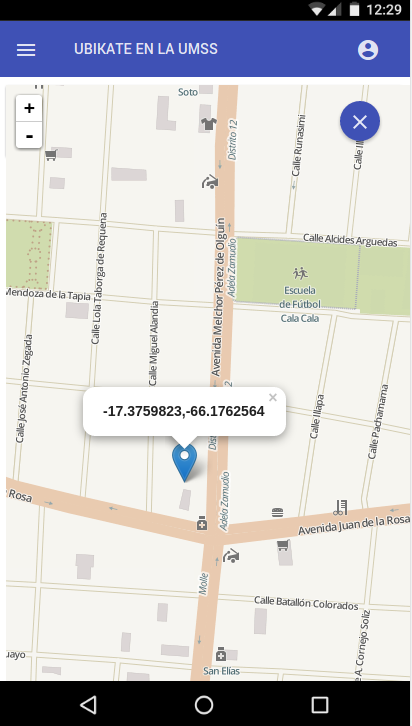
\includegraphics[width=0.3\textwidth]{iteration2/location_marker}
    \caption{Tooltip con la latitud y longitud de la posición actual del usuario.}
    \label{fig:location_marker}
    \caption*{Fuente: Elaboración propia.}
  \end{center}
\end{figure}


% \subsubsection{Manejo de Usuarios}
% \label{sub:Manejo de Usuarios}
%
% Si se quiere saber la ruta más corta entre el usuario y un lugar conocer la locación del usuario, hay que tomar en cuenta que esta información no se encuentra en la base de datos, es necesario obtener el punto georreferenciado del usuario como punto de inicio, para lo cual se utilizó el API de geolocalización propio de HTML5, la especificación de HTML5 indica que el navegador puede acceder y usar los recursos nativos de un smartphone pero es necesaria la aceptación del usuario mediante un mensaje que el navegador despliega, la locación es encontrada mediante la triangulación de Coordenadas por GPS (el mas exacto a la hora de encontrar la locación del dispositivo), Wi-Fi, GSM o CDMA. Solo es necesaria la ejecución de la siguiente línea para poder obtener la posición actual del usuario usando el API de geolocalización de HTML5. \\
%
% \begin{verbatim}
%   var coords = Geolocation.getCurrentPosition();
%   var latitud = coords.latitude;
%   var longitud = coords.longitude;
% \end{verbatim}
%
% La \emph{latitud} y \emph{longitud} obtenidas es fácilmente trasladado al mapa usando \emph{ember-leaflet} mediante un marcador, como se puede apreciar en la siguiente figura.
%
% \begin{figure}[H]
%   \begin{center}
%     \caption{Tooltip con la latitud y longitud de la posición actual del usuario.}
%     \label{fig:location_marker}
%     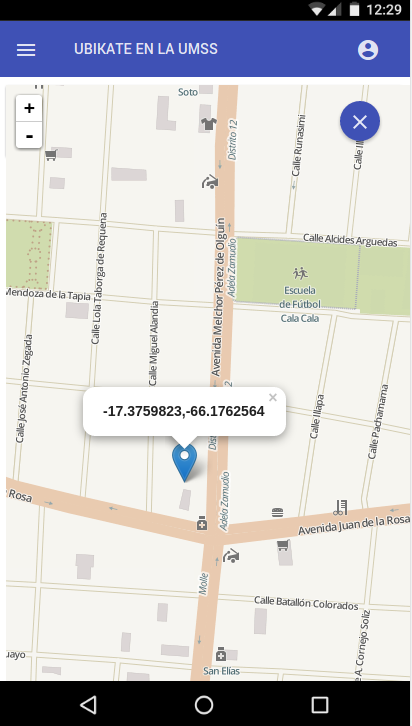
\includegraphics[width=0.5\textwidth]{iteration2/location_marker}
%     \caption*{Fuente: Elaboración propia.}
%   \end{center}
% \end{figure}



\subsubsection{Mostrar los Rutas}
\label{sub:Mostrar los Rutas}

Para dibujar líneas rectas sobre un mapa hay que tomar en consideración que la tierra no es plana y las líneas que en un mapa parecen líneas rectas, realmente no son rectas, ya que el planeta Tierra es un \emph{esferoide oblato}\footnote{Un \emph{esferoide oblato} (o elipsoide oblato) es un elipsoide de revolución obtenido por rotación de una elipse alrededor de su eje más corto.} por lo que las líneas en apariencia rectas tienen la curvatura natural del planeta Tierra. En distancias largas esto tiene un gran impacto al manejar o utilizar mapas proyectados, pero también es cierto que para una área pequeña como es el campus de la Universidad de San Simón este problema no tiene un gran impacto pero no está demás en tomar en cuenta esta característica en el análisis de datos geoespaciales, como se explicó en el capitulo \ref{cha:geolocalizacion}, para el presente proyecto se usará el proyección \emph{SRID 3857}.\\


% \section{Ruta óptima dentro el Campus Universitario}
% \label{sec:generar_mapa_rutas}

En resumen, para responder al problema de encontrar una ruta óptima entre 2 puntos dentro del campus universitario, se necesita de un mapa que contenga todas las rutas que existen dentro del campus.\\

 %
 %
 % \section{Campus Universitario}
 % \label{sec:ruta_corta_umss}

 En primer lugar fue necesario obtener un grafo ponderado no-dirigido que representa un mapa de los caminos que existen dentro del campus Universitario.\\

 Para obtener este mapa se procedió a caminar a través del campus de la UMSS con un GPS Garmin Nuvi 1300, el cual es un dispositivo GPS básico pero cumple con la función de guardar información geográfica, los archivos generados tienen extensión \emph{gpx}, que básicamente es un fichero XML estándar usado para compartir datos entre GPS's, se recorrieron los principales caminos que existen e interconectan las distintas facultades y oficinas dentro del campus universitario. Una vez realizado este recorrido, se procedió a extraer la información del dispositivo GPS, se utilizó el archivo \emph{current.gpx} para exportar la información  a un archivo \emph{shapefile}, para esta tarea se utilizó QGis, con el cual se acabó editando las rutas recogidas por el GPS.\\

% \footnote{Un shapefile es un archivo de formato sencillo y no topológico que se utiliza para almacenar la ubicación geométrica y la información de atributos de las entidades geográficas.\cite{what_is_shapefile} }

 Este paso fue necesario porque el mapa extraído del GPS es una línea única, pero para que nos sirva para el objetivo de buscar una ruta óptima, es necesario que esta línea sea dividida o separada en muchas líneas, las cuales son las aristas y los extremos de las líneas serán los nodos o vértices del grafo.\\

 Implementando el algoritmo de \emph{Dijkstra} en el grafo resultante es lo que nos permitir\'a encontrar la ruta más corta dentro del campus Universitario, al tener una gran cantidad de información resultante de la obtención de datos mediante un dispositivo GPS se hace imprescindible usar una base de datos que nos ayude con esta tarea, para lo cual se usó la base de datos PostgreSQL añadiendolo PostGIS y pgRouting, herramientas ampliamente utilizadas en el manejo de datos geo-espaciales.\\

  % el grafo representa el mapa de caminos  pueda ser usado en una base de datos  “ruteable”, esto significa que el mapa de una sola línea hay que separarlo o dividirlo en muchas líneas.\\


 Técnicamente esta línea única es representada como un \emph{POLYLINE} el cual consiste en una o más partes. Una parte es una secuencia conectada de dos o más puntos. Las partes pueden o no estar conectadas entre sí. Las partes pueden o no intersectarse entre sí, para transformar este POLYLINE necesitamos separar todas sus partes y convertirlas en objetos \emph{LINESTRING} únicos, y a este conjunto de LINESTRINGs es el que se va a usar en la base de datos como mapa de ``rutas''.\cite{esri_shapefile}\\

 \begin{figure}[H]
   \begin{center}
     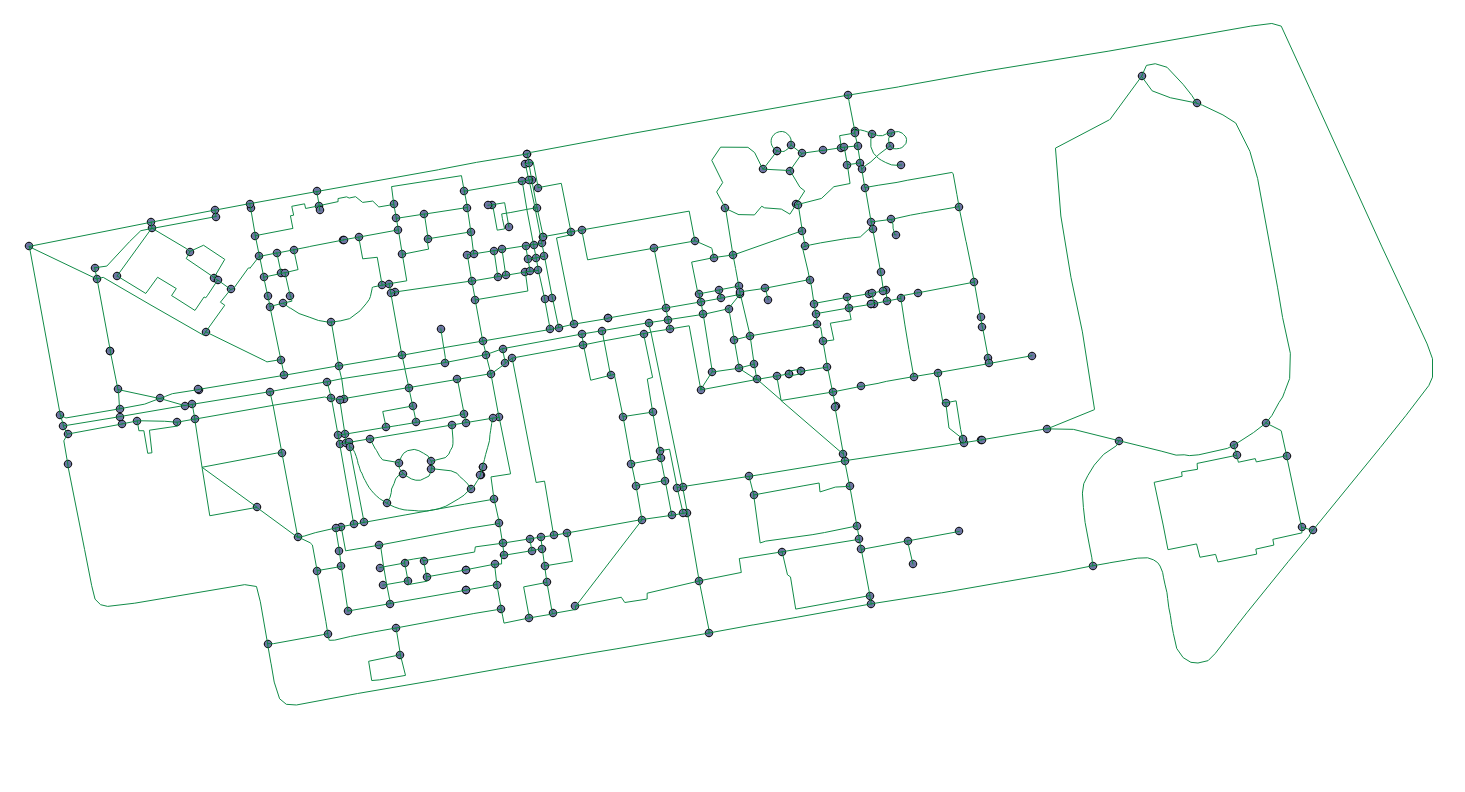
\includegraphics[width=1\textwidth]{shapefile_umss_v1}
     \caption{Shapefile del campus Universitario.}
     \label{fig:shapefile_umss_v1}
     \caption*{Fuente: Elaboración propia}
   \end{center}
 \end{figure}

 En la figura \ref{fig:shapefile_umss_v1} se puede apreciar el shapefile resultante de la división del POLYLINE original, las líneas que conforman el mapa de las rutas del campus Universitario, donde cada línea es una arista y los puntos son los nodos del grafo no-dirigido, que será usado para la resolución del problema de la ruta más corta en el presente proyecto de grado.\\
 %
 % Para una mejor apreciación del grafo que consta de 1164 aristas y 1003 vértices, se lo puede ver en combinación o proyectada en un mapa de rutas del campus de la Universidad Mayor de San Simón ubicado entre las calles Oquendo, Sucre y  Belzu de la ciudad de Cochabamba - Bolivia, se puede referir a la siguiente figura \ref{fig:shapefile_umss_v2}.
 %
 % \begin{figure}[H]
 %   \begin{center}
 %     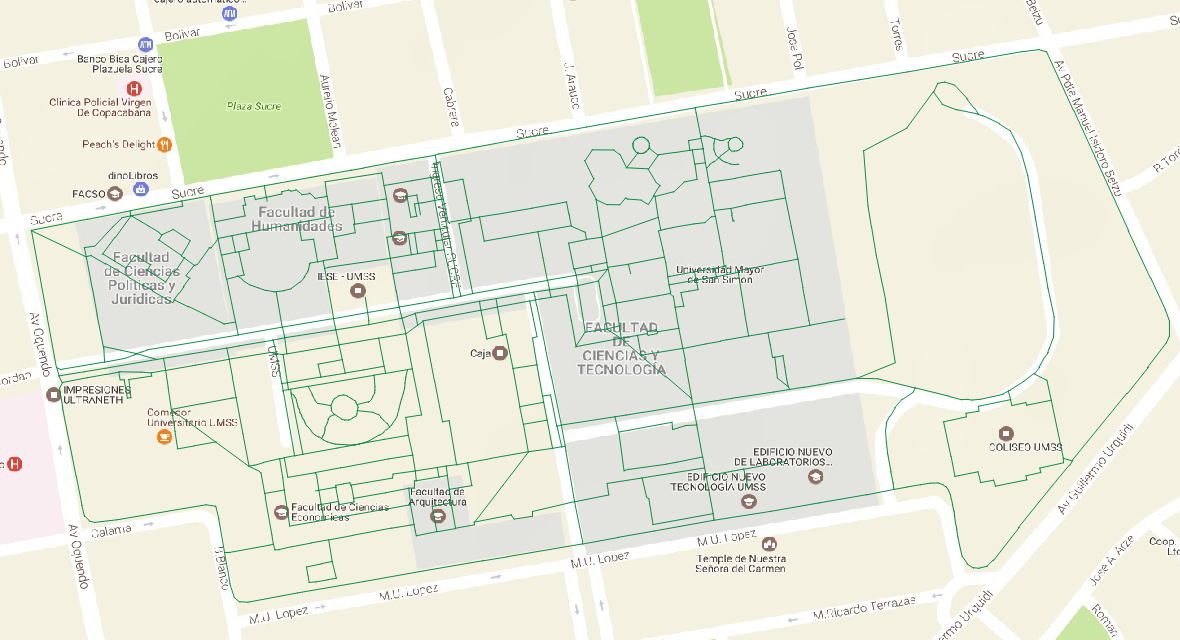
\includegraphics[width=1\textwidth]{shapefile_umss_v2}
 %     \caption{Shapefile sobre el campus Universitario de la UMSS.}
 %     \label{fig:shapefile_umss_v2}
 %     \caption*{Fuente: Elaboración propia}
 %   \end{center}
 % \end{figure}


% \subsubsection{Las Rutas}
% \label{subs:Las Rutas}

Después de generar el archivo shapefile, se procede a popular la base de datos del mismo modo que se hizo con la información de los lugares. Para las rutas se genera una tabla nombrada \emph{ways}.\\

Posteriormente se procede a preparar la tabla \emph{ways} para que soporte las funciones instaladas por pgRouting.
% Una vez poblada la base de datos se procede a cargar la misma con la información obtenida en RF011, para tal efecto es necesario primeramente crear una tabla que contendrá los LINESTRING contenidos en el shapefile, esta operación es similar a la realizada en la tarea - RF003 (\ref{sub:RF003}). Una vez que ya se tiene la tabla a la llamamos \emph{ways},
Es necesario ejecutar un query propio de \emph{pgRouting} el cual tiene como objetivo analizar los datos geo-espaciales de la tabla y añadirle una \emph{topología}.\\

\begin{verbatim}
  select pgr_createTopology('ways', 0.00000001, 'geom', 'gid');
\end{verbatim}

Dentro lo que es la \emph{topología geoespacial} existe una aplicación que se lo conoce como \emph{topología de red}. La \emph{topología de red} representa las relaciones entre segmentos en una red lineal o una colección de segmentos de línea. \cite{osgeo_journal_topology} \\

En un \emph{SIG} la topología ayuda a mejorar el análisis de datos geo-espaciales, para resolver el problema de la ruta corta \emph{pgRouting} genera una \emph{topología de red} usando los datos que existen en la tabla \emph{ways}, es necesario ejecutar una instrucción, la que se muestra a continuación y \emph{pgRouting} se encarga de llenar los datos que se pueden observar en la figura \ref{fig:postgres_ways}, las columnas \emph{source} y \emph{target} son populadas con el análisis topológico y en la figura \ref{fig:postgres_vertices}, se puede observar que la tabla \emph{ways\_vertices\_pgr} es creada enteramente en la ejecución de la instrucción.\\

\begin{figure}[H]
  \begin{center}
    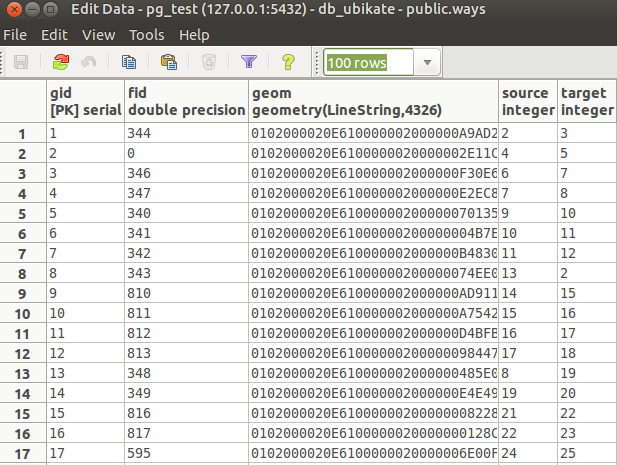
\includegraphics[width=0.8\textwidth]{iteration2/postgres_ways}
    \caption{Vista de la tabla \emph{ways}.}
    \label{fig:postgres_ways}
    \caption*{Fuente: Elaboración propia}
  \end{center}
\end{figure}

En la figura \ref{fig:postgres_ways} se puede apreciar que cada fila es una parte de la línea original obtenida por el dispositivo GPS y explosionada por QGIS, hay que notar que las columnas \emph{source} y \emph{target} hacen referencia a los nodos o vértices que la primera línea tiene en sus extremos, la primera línea o fila está identificada por la columna \emph{gid}.\\

En la siguiente figura \ref{fig:postgres_vertices} se observa la tabla \emph{ways\_vertices\_pgr} que contiene los vértices creados a partir del análisis de los datos en la tabla \emph{ways}.

\begin{figure}[H]
  \begin{center}
    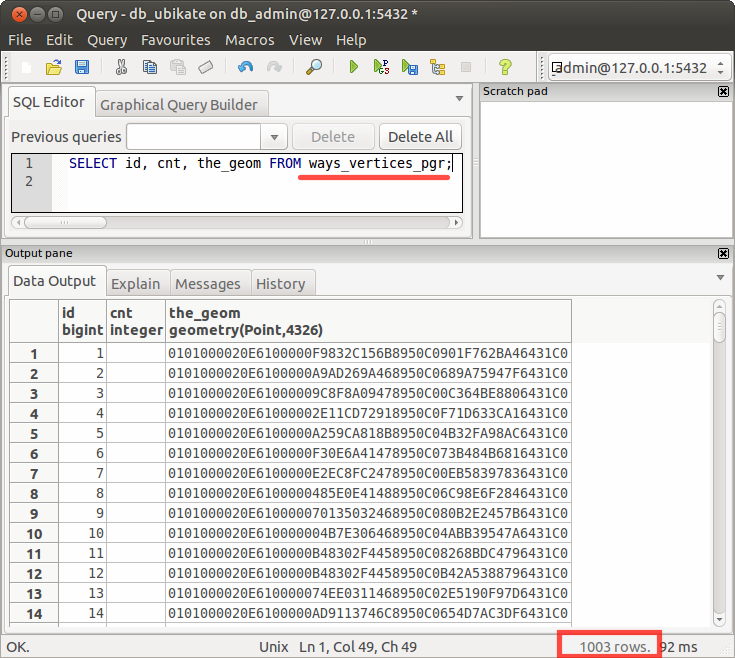
\includegraphics[width=0.8\textwidth]{iteration2/postgres_vertices}
    \caption{Vista de la tabla \emph{ways\_vertices\_pgr}.}
    \label{fig:postgres_vertices}
    \caption*{Fuente: Elaboración propia}
  \end{center}
\end{figure}

Para entender los datos generados hay leer la información de las 2 tablas, por ejemplo en la primera  fila (gid 1) de la tabla \emph{ways}, se observa que el contenido de la columna \emph{source} es igual a \textbf{2} y \emph{target} es igual a \textbf{3}, eso quiere decir que los vértices del LINESTRING de la fila 1 son los vértices con \textbf{id} 2 y 3 respectivamente de la tabla \emph{ways\_vertices\_pgr}.\\


Todo el conjunto de vértices y líneas de estas tablas se podría representar con una Matriz de adyacencias, explicada en \ref{sub:representacion_de_un_grafo}, y usada en la resolución de la ruta mas corta, mas específicamente con el algoritmo de Dijkstra.\\

\begin{center}
  \begin{lstlisting}[label=pgr_dijkstra,caption=Algoritmo de Dijkstra implementado en \emph{pRouting}]
    SELECT seq, id1 AS node, id2 AS edge, cost
    FROM pgr_dijkstra(SELECT gid AS id,
                              source::integer,
                              target::integer,
                              st_length(geom) AS cost
                       FROM public.ways, targetId, sourceId, false, false);
  \end{lstlisting}
\end{center}


La anterior consulta SQL es una llamada al método \emph{pgr\_dijkstra} implementado en \emph{pgRouting} el cual solo puede ser utilizado una vez que la base de datos está preparada para tal efecto, es decir necesitamos que la tabla de rutas \emph{ways} tenga la topología de red y también es necesario los ids de los nodos de destino y origen, \emph{targetId} y \emph{sourceId} respectivamente, estos dos últimos datos son obtenidos por una combinación de acciones ya que los nodos son propios del mapa de rutas y el punto destino es en realidad un lugar el cual está ubicado en otra tabla y el punto origen es donde se encuentra el cliente dentro del campus Universitario, por lo tanto una vez obtenido los punto geo-referenciados del lugar de la tabla \emph{places} y el punto donde se encuentra parado el cliente se obtienen los nodos ``más'' cercanos a estos puntos, gracias a que \emph{PostGIS} ya lo tiene implementado, encontrar el nodo más cercano es tan fácil como ejecutar la siguiente consulta SQL, donde \emph{lon} y \emph{lat} son la longitud y latitud del lugar.

\begin{verbatim}
    SELECT id
    FROM ways_vertices_pgr
    ORDER BY the_geom <-> ST_GeometryFromText('POINT(lon lat)', 3857)
    LIMIT 1
\end{verbatim}

Una vez ejecutado el método \emph{pgr\_dijkstra} se obtiene un conjunto de líneas, que son un conjunto de latitudes y longitudes que representa la ruta más corta entre el punto origen y el punto destino, esta informacion realmente no dice nada a la persona que lo lee por lo tanto requiere ser procesada para poder ser consumida desde el navegador, este proceso es llevada a cabo en el servidor y entregada al cliente en formato GeoJSON.\\







En el navegador, se obtiene
% poder mostrar la ruta óptima es necesario obtener
de la base de datos un conjunto de datos en formato de latitud y longitud que conforman líneas, las cuales representan la ruta más corta, pero al final es solo un montón de números, sin mucho significado para el usuario, toda esta información es difícil de procesar y el usuario necesita información que sea fácil de entender y no existe mejor herramienta disponible para esta tarea que mostrar la \emph{ruta} de forma visual, esto quiere decir que se necesita mostrar la ruta sobre un \emph{mapa}, ya que en la aplicación se implementó \emph{ember-leaflet} para desplegar el mapa y mostrar un lugar, también se puede  mostrar más ruta más corta mediante una línea, a la que también se puede personalizar (la línea se muestra de color rojo).\\

A continuación se puede apreciar el \emph{request} que el frontend hace al API y  el objeto GeoJSON que es recibido, este objeto contiene la información geoespacial necesaria para ``dibujar'' la línea roja entre 2 puntos georeferenciados, uno de los puntos es donde se encuentra el usuario (\emph{sourceData}) y el otro punto es el lugar (\emph{targetData}).
% A continuación se puede apreciar el request al API

 % uno de los cuales es el lugar al que se quiere llegar y el otro es la ubicación actual del usuario. \\

\begin{verbatim}
  ENV.APP.API_HOST + '/api/v1/ways/route/' + sourceData.id + '/' + targetData.id;

  GET /api/v1/ways/route/930/77 200 276.217 ms - 3911

  $ curl http://localhost:3000/api/v1/ways/route/930/77 | python -m json.tool                                                       [3:04:52]
  % Total    % Received % Xferd  Average Speed   Time    Time     Time  Current
                                 Dload  Upload   Total   Spent    Left  Speed
100  3911  100  3911    0     0   161k      0 --:--:-- --:--:-- --:--:--  166k
{
    "features": [
        {
            "geometry": {
                "coordinates": [
                    [
                        -66.1467397848201,
                        -17.3935321732846
                    ],
                    [
                        -66.1467190789842,
                        -17.3935294725234
                    ]
                ],
                "type": "LineString"
            },
            "type": "Feature"
        },

\end{verbatim}
% /api/v1/ways/route/

Una vez que se tiene los datos, es necesario representarlo en el mapa y para tal efecto se seguirá utilizando \emph{ember-leaflet} y que con el siguiente \emph{tag}, se puede observar en el mapa una línea roja que representa la ruta más corta,  entre el punto donde se encuentra el usuario y el punto del lugar a buscar. Tal como se puede apreciar en la figura \ref{fig:short_way_place}.
% Este objeto es representado en el mapa usando ember-leaflet con la siguiente instrucción,
%
\begin{verbatim}
  {{#geojson-layer geoJSON=currentGeoJSON color='red' }}
\end{verbatim}

% Se puede

\begin{figure}[H]
  \begin{center}
    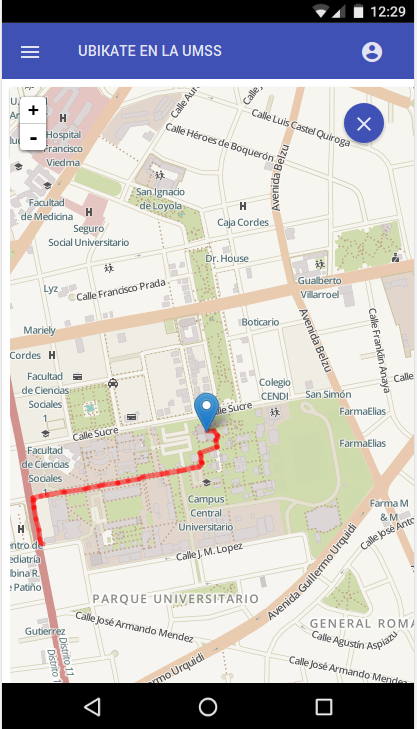
\includegraphics[width=0.5\textwidth]{iteration2/short_way_place}
    \caption{Ruta más corta dibujada con una línea roja.}
    \label{fig:short_way_place}
    \caption*{Fuente: Elaboración propia.}
  \end{center}
\end{figure}



% Para dibujar líneas rectas sobre un mapa hay que tomar en consideración que la tierra no es plana y las líneas que en un mapa parecen líneas rectas, realmente no son rectas, ya que el planeta Tierra es un \emph{esferoide oblato}\footnote{Un \emph{esferoide oblato} (o elipsoide oblato) es un elipsoide de revolución obtenido por rotación de una elipse alrededor de su eje más corto.} por lo que las líneas en apariencia rectas tienen la curvatura natural del planeta Tierra. En distancias largas esto tiene un gran impacto al manejar o utilizar mapas proyectados, pero también es cierto que para una área pequeña como es el campus de la Universidad de San Simón este problema no tiene un gran impacto pero no está demás en tomar en cuenta esta característica en el análisis de datos geoespaciales, como se explicó en el capitulo \ref{cha:geolocalizacion}, para el presente proyecto se usará el proyección \emph{SRID 3857}.\\


\subsection{Registrar el Avance}
\label{sub:iteracion2_avance}

% \subsection{Verificación}
% \label{sub:iteracion2_verificacion}
